\chapter{Custom Environments}\label{chp:custom_envs}
This chapter explains how to create a custom environment for use with VTOL-AirSim. Like the previous chapter on custom aircraft, this chapter is structured as a guide through a specific example that demonstrates the complete process starting with obtaining assets from the Unreal Engine Marketplace to a full VTOL-AirSim simulation in the new environment.

We begin with a discussion on obtaining assets from the Unreal Engine Marketplace. The proceeding sections are a guide through a specific example in which we first create a new Unreal Project, then we add to the project Unreal Engine assets from the marketplace, and finally we add the VTOL-AirSim Plugin.

\section{Unreal Engine Marketplace}
The easiest way to create a custom environment is by downloading a prebuilt environment from the Unreal Engine Marketplace, found at \url{https://unrealengine.com/marketplace}. In contrast to an aircraft in VTOL-AirSim, which is a small mesh made up of a few moving parts, an environment is much larger, and is typically composed of a great number of meshes and other details such as lighting, sky objects, bodies of water, and dynamic actors arranged in a complex layout. Creating an environment --- or a \textit{level}, as it is called in UE4 --- on one's own requires a deep understanding of Unreal Engine to do well. However, if you are able to obtain a level that is already made, the process is very simple.

The Unreal Engine Marketplace has a large selection of assets available to download. Many of them are paid, though there is a significant amount of free assets to choose from. The assets on the marketplace are of all types of UE4 assets, including Materials, Textures, Static Meshes, Blueprints, etc., so you must be careful in that you choose a product that contains one or more levels among the provided assets. Study the product's description to know whether it comes with a prebuilt level. As an example, the images for a product could be pictures of different types of buildings with scenic backgrounds, yet the product simply contains an assortment of buildings, without any levels containing those buildings. These are assets that are meant to be used by creators who are designing their own levels. Note that you may find levels referred to as \textit{maps} in product descriptions, due to level assets having the file extension \ci{.umap}. Also, some products do come with prebuilt levels but simply fail to mention this in their descriptions, so you can also check the \textbf{Reviews} and \textbf{Questions} tabs when viewing a product for more clues.

When searching for assets, you also need to choose assets that are compatible with the version of Unreal Engine which you are using. You can filter results while searching for assets on the UE Marketplace by clicking the label of your version in the \textbf{Filter Results} column under \textbf{Supported Engine Versions}.

\section{Obtain Assets from Unreal Engine Marketplace}\label{sec:obtain_assets_windows}
As of this writing, the only way to download assets obtained on the UE Marketplace is through the \textit{Epic Games Launcher}, and it is only available for Windows or MacOS. While it is theoretically possible to use the Epic Games Launcher on Linux using the compatibility layer \textit{Wine}, that is outside the scope of this text. The example in this chapter has only been tested using Windows, so we will provide instructions for Windows only.

The Epic Games Launcher and Unreal Engine on Windows are free software, so all you need is access to a machine, hard drive, partition, or virtual machine that has an instance of Windows for which you have internet access and admin rights to download and install software. You also need at least 40 GB of free space available in Windows.

\subsection{Install The Epic Games Launcher and Unreal Engine (Windows)}

On Windows, go to \url{https://epicgames.com/store/en-US/download} to download the Epic Games Launcher installer. Install it and open it. When it opens, it will ask you to sign in to your Epic account. Sign in using your Epic Games account (you should already have one if you've done the steps in Section~\ref{sec:unreal_requirements}). Next, click on the \textbf{Library} tab. Click the plus icon next to \textbf{Engine Versions} to install a version of Unreal Engine (Fig.~\ref{fig:egl_ue_version}). Click on the version number then select whichever version is compatible with AirSim; at the time of this writing, it is Unreal Engine version 4.25. Note that the last number in the version label, called the patch version, doesn't determine compatibility, so just choose the highest patch version, which is 4.25.4 at the time of this writing. Once you have chosen a version, click \textbf{Install}. The download and installation will take a while complete.

\begin{figure}[h]
    \centering
    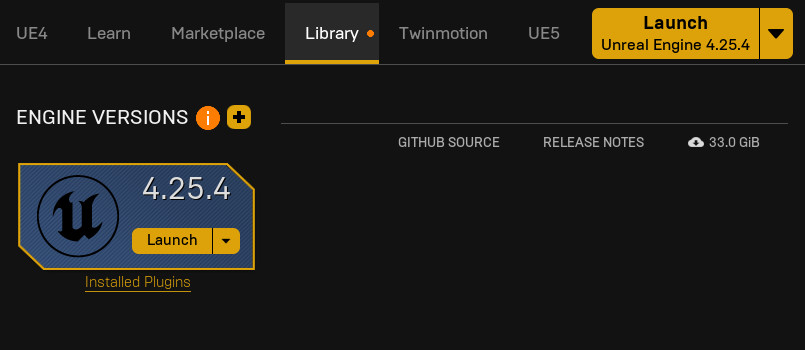
\includegraphics[width=\textwidth]{figures/egl_ue_version2.jpg}
    \caption[Epic Games Launcher: Install Unreal Engine]{
        The Epic Games Launcher with Unreal Engine 4.25.4 installed.}%
    \label{fig:egl_ue_version}
\end{figure}

\subsection{Create a New Unreal Project (Windows)}
When the installation of Unreal Engine has finished, click \textbf{Launch} to start Unreal Editor. You will be presented with a window after it initializes. Create a new project by doing the following: select \textbf{Games} and click \textbf{Next}, then select \textbf{Blank} and click \textbf{Next}, then click \textbf{With Starter Content} and change it to \textbf{No Starter Content}, and finally give it the name \ci{CoolBridge} and click \textbf{Create Project}.

\subsection{Download Assets from Marketplace (Windows)}
You can explore the UE Marketplace from either a web browser or within the Epic Games Launcher. Let's do so with the Epic Games Launcher, as it allows for direct downloading of assets into an Unreal Project. In the Launcher, click the \textbf{Marketplace} tab. We are going to download a free asset bundle named \textit{Automotive Bridge Scene} from Epic Games. Search for it using the search bar, and it should be the top or the only result. Click on the product image, then click the button that says \textbf{Free} to access it. Once it is yours, click \textbf{Add to Project}, then in the pop-up select the \ci{CoolBridge} project and click \textbf{Add to Project}. Wait for it to install to your project, then close out of the Epic Games Launcher and Unreal Engine once it finishes.

\begin{figure}[h]
    \centering
    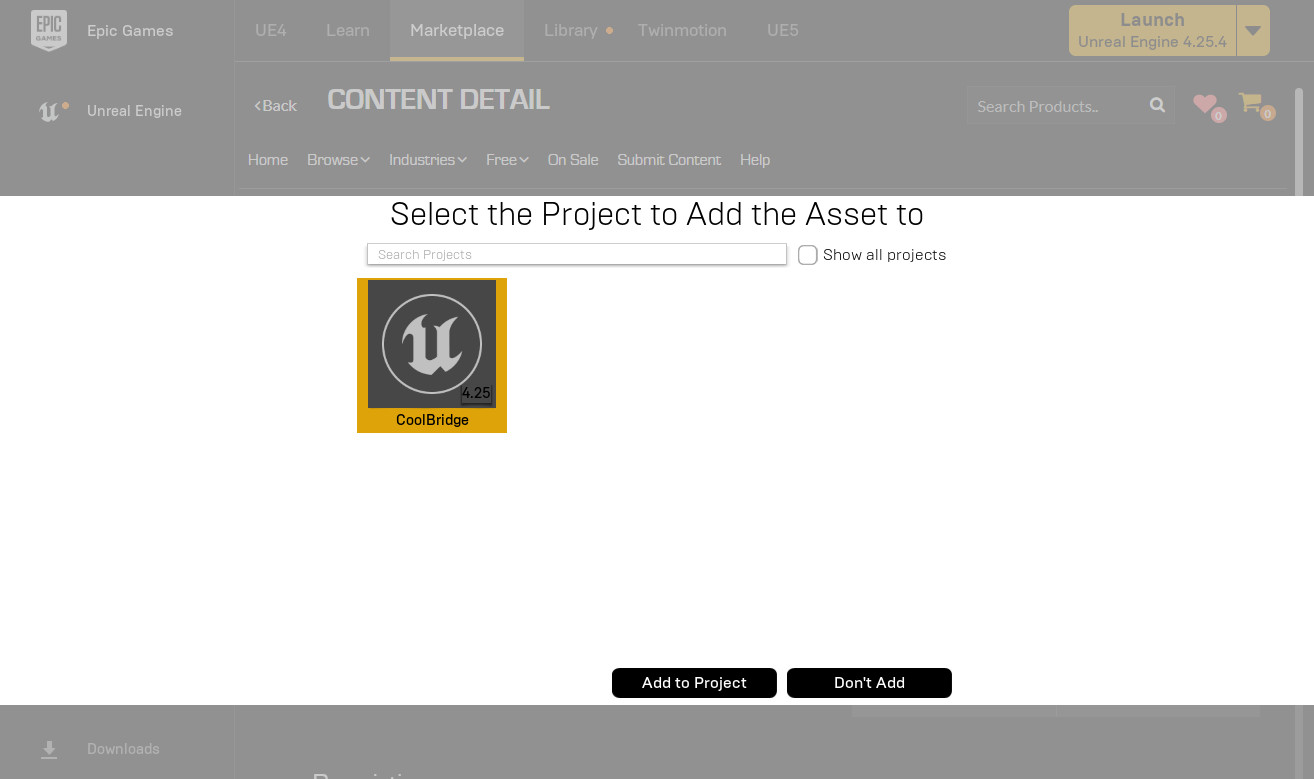
\includegraphics[height=225pt]{figures/egl_add_to_project_edit}
    \caption[Epic Games Launcher: Download assets to project]{
        In the Epic Games Launcher, this is the screen that allows you to download assets to a project.}%
    \label{fig:egl_add_to_project}
\end{figure}

As a final step, navigate to the Windows directory where the \ci{CoolBridge} project is located. By default, this should be in your \ci{Documents} folder under \ci{Unreal Projects}. If you look inside the \ci{Content} folder of the project, you'll notice that there is a folder named \ci{AutomotiveBridgeScene}. Note that this folder contains all of the assets that were just downloaded from the marketplace. Now go back to the \ci{CoolBridge} folder and delete the folders \ci{Intermediate}, \ci{Binaries}, \ci{Saved}, \ci{.vs}, and the file \ci{CoolBridge.sln}, if they are present.

That is all we needed to do using Windows. The remaining steps will all be done in Linux.

\subsection{Set the Project Up on Linux}
Copy the \ci{CoolBridge} folder to your Linux file system and place it in a directory of your choice. Create a folder in \ci{CoolBridge} named \ci{Plugins}, and place inside it a working copy of VTOL-AirSim (i.e., not broken) from one of your other Unreal Projects.

\section{Edit Project in Unreal Editor}\label{sec:edit_project_ueditor}
Launch Unreal Editor and open the \ci{CoolBridge.uproject} file. In the dialog, select \textbf{More Options} then \ci{Convert in-place}, and it will convert your project to work with your version of Unreal Engine on Linux. On the next dialog, click \textbf{Yes} to rebuild the modules.

When the project has been built and is opened in the editor, you should get a notification in the bottom-right that says \textit{Project file is out of date. Would you like to update it?} Select \textbf{Update}, and this will add an entry to the \ci{CoolBridge.uproject} file that contains the AirSim Plugin as part of the project. Also, before proceeding, go to \textbf{Edit > Editor Preferences}, and in the search box, type \texttt{CPU} and ensure that the setting \textbf{Use Less CPU when in Background} is unchecked.

In the \textbf{Content Browser}, navigate to the folder \ci{AutomotiveBridgeScene/Maps} and double-click on the level \ci{Bridge_P}. This will load the level in the editor. It may take a while to load the first time. When the Editor has loaded the level and finished compiling the necessary shaders, you should see a picturesque scene of a bridge in the \textbf{Level Viewport}.

\subsection{Configure the Project for VTOL-AirSim}
Let's make this level the default one in case we want to package it into a standalone application later. Go to \textbf{Edit > Project Settings}, then click \textbf{Maps \& Modes} in the left column. Change both the \textbf{Editor Startup Map} and the \textbf{Game Default Map} to be the current level, \ci{Bridge_P}. Close out of the project settings.

Next, in order to perform a VTOL-AirSim simulation when we use Play In Editor or when we launch the standalone application, we have to set the \textit{Game Mode} to be \ci{AirSimGameMode}. Do that by going to \textbf{Window > World Settings}, then in the \textbf{World Settings} panel in the lower-right corner, find the \textbf{GameMode Override} setting and change it to \ci{AirSimGameMode}.

\subsection{Place a Player Start Actor}

\begin{figure}[t]
    \centering
    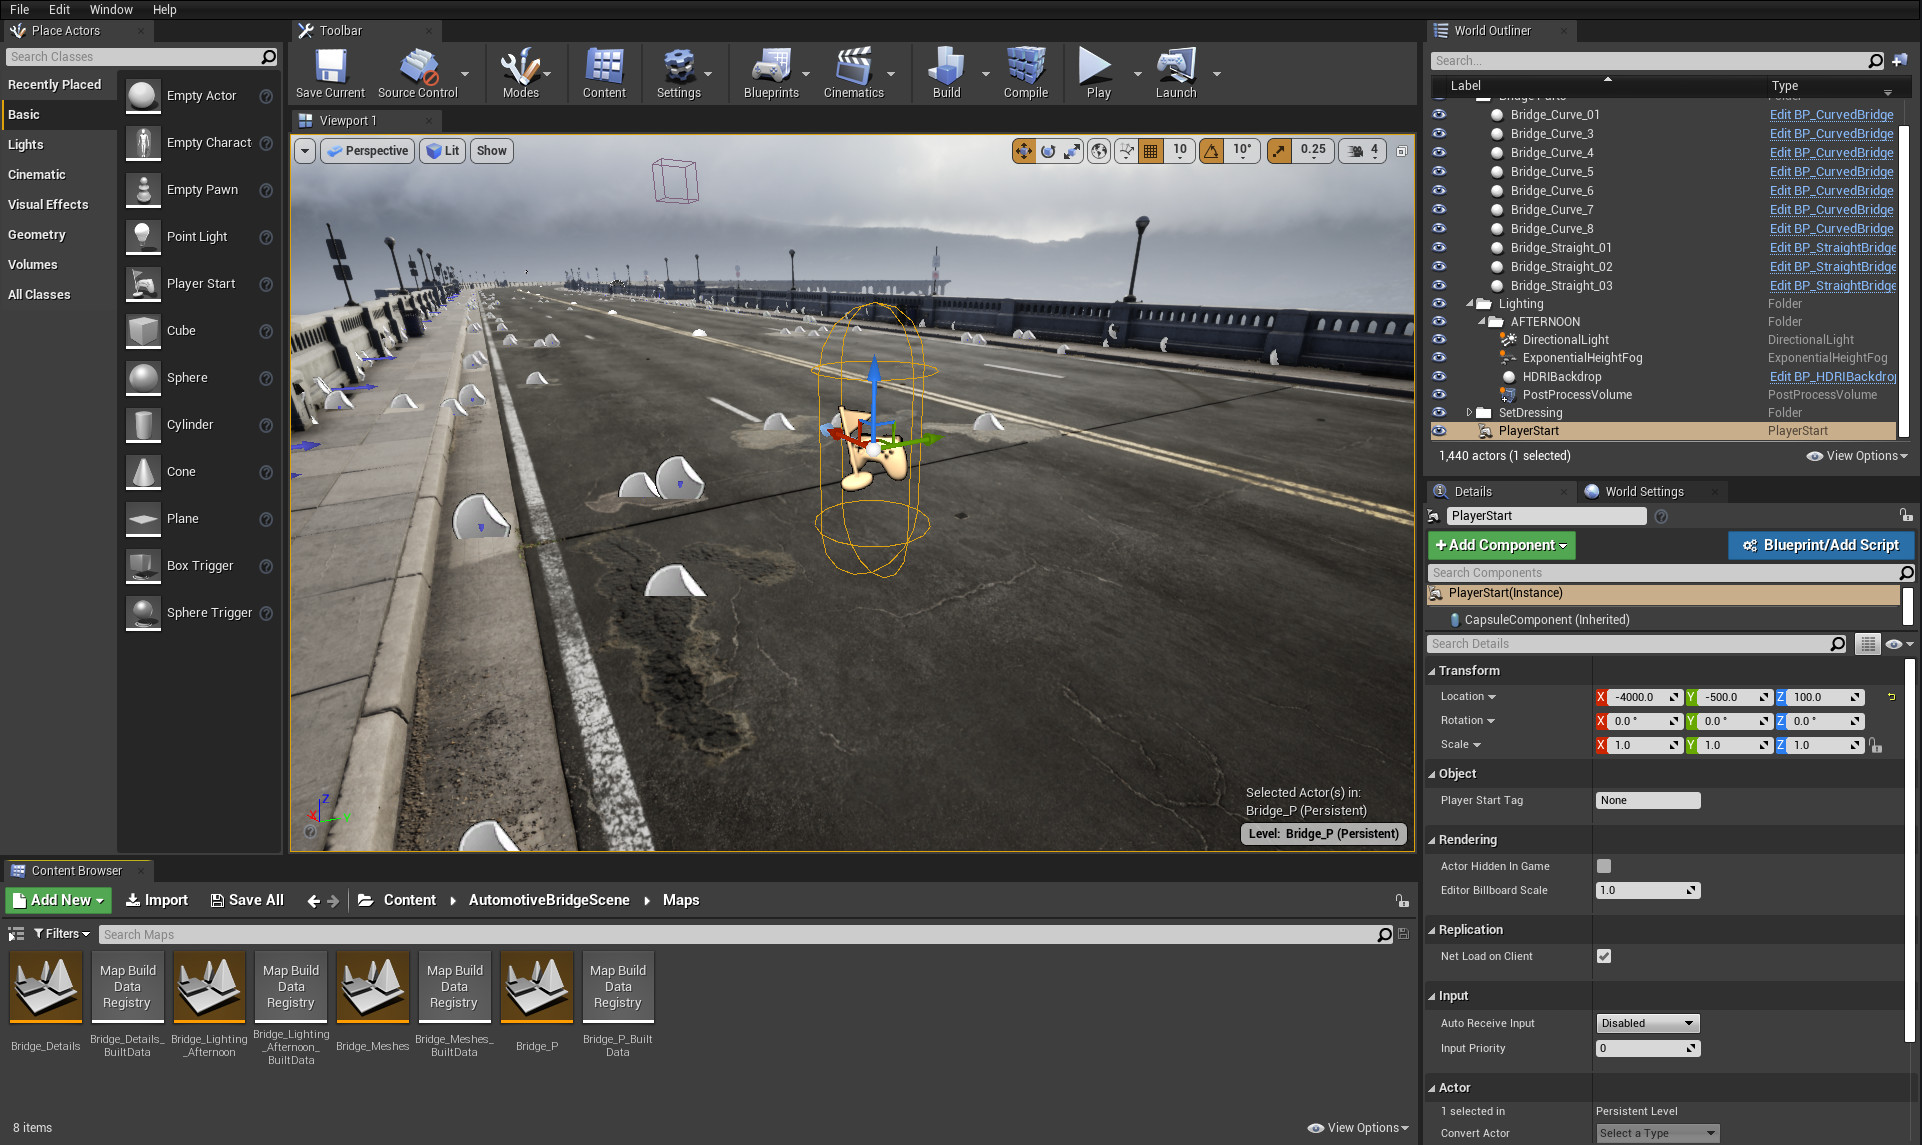
\includegraphics[width=\textwidth]{figures/ue4_bridge_playerstart}
    \caption[Custom environment in Unreal Editor]{
        The custom environment with a \textbf{Player Start} actor placed in the level.}%
    \label{fig:ue4_bridge_playerstart}
\end{figure}

Now we need to set where we want the vehicle to spawn in the world --- or, more precisely, where we want the global origin to be for VTOL-AirSim. \ci{AirSimGameMode} is configured to look for the \textbf{Player Start} Actor to set the global origin and spawn the vehicle; however, there is no \textbf{Player Start} Actor in this level, so we need to add one. In the \textbf{Place Actor} panel, find \textbf{Player Start} and drag it onto the \textbf{Level Viewport}. It should now appear in the \textbf{World Outliner} panel, and it should also have its attributes visible in the \textbf{Details} panel. While you may set the \textbf{Player Start} Location to wherever you like, we found a good starting position for this example to be the Location (X, Y, Z) values of (-4000.0, -500.0, 100.0). Set the \textbf{Player Start}'s Location attribute to be these values. You can double-click on the \ci{PlayerStart} Actor in the \textbf{World Outliner} to center the \textbf{Level Viewport} over its new location. After centering the view, the \textbf{Level Viewport} should look similar to Fig.~\ref{fig:ue4_bridge_playerstart}.

\section{Flight in New Environment}
We are ready to fly the tiltrotor aircraft in the level. First, make sure your settings file at the path \ci{~/Documents/settings.json} is set with \ci{"SimMode": "Vtol"}. Next, press \textbf{Play} in the editor, and in the \textbf{Level Viewport} you should see the tiltrotor aircraft spawn in the level. In a terminal, run the geometric controller example from Section~\ref{sec:vtol_geometric_control}. You should now see the tiltrotor flying through the custom environment, as shown in Fig.~\ref{fig:ue4_bridge_flying}.

\begin{figure}[h]
    \centering
    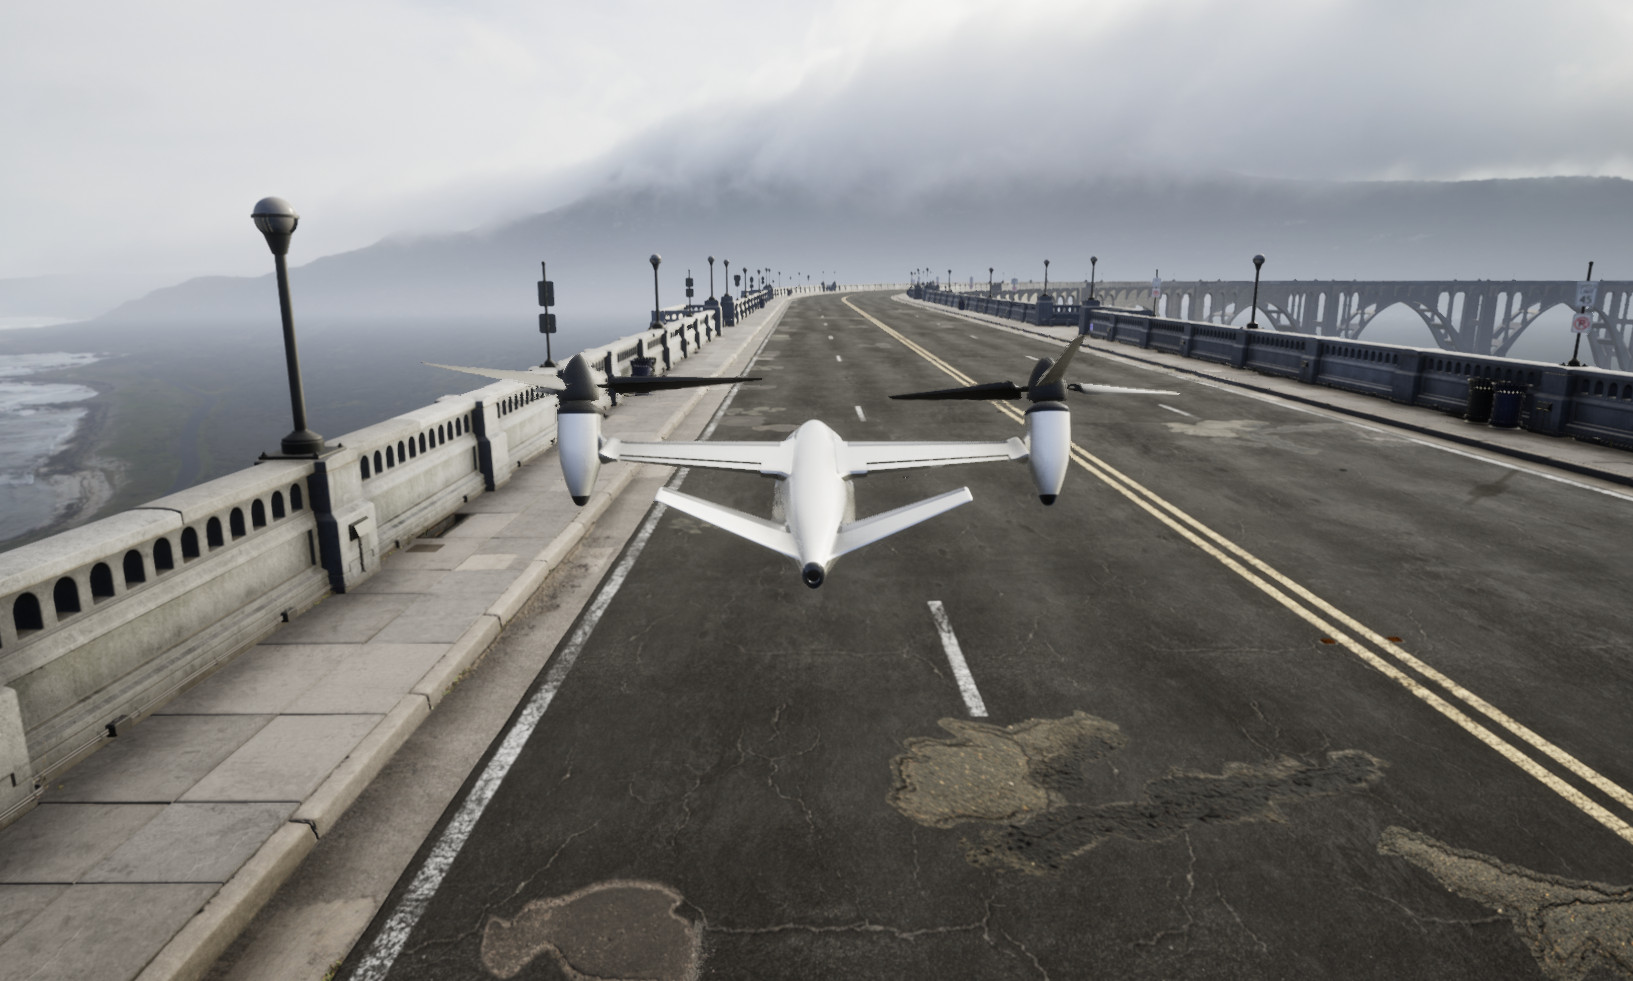
\includegraphics[width=\textwidth]{figures/ue4_bridge_flying}
    \caption[Tiltrotor flying in custom environment]{
        The tiltrotor aircraft flying in the \textit{Automotive Bridge Scene} custom environment.}%
    \label{fig:ue4_bridge_flying}
\end{figure}